\documentclass[11pt]{article}
\usepackage[margin=1in]{geometry}
\usepackage{amsmath,amssymb}
\usepackage{listings}
\usepackage{booktabs}
\usepackage{graphicx}
\usepackage{hyperref}
\usepackage{xcolor}
\usepackage{tikz}
\usetikzlibrary{arrows.meta,positioning,calc}

\lstset{
  basicstyle=\ttfamily\small,
  keywordstyle=\color{blue!70!black}\bfseries,
  commentstyle=\color{green!50!black}\itshape,
  stringstyle=\color{red!60!black},
  breaklines=true,
  frame=single,
  framesep=3pt,
  columns=fullflexible,
  xleftmargin=1em,
  xrightmargin=1em,
}

\title{Syntax-Directed SOP Decomposition\\
       for BDD-Based Logic Synthesis}
\author{SV Toolkit Technical Report}
\date{March 2026}

\begin{document}
\maketitle

\begin{abstract}
We describe the SOP (sum-of-products) equation output tool for the SV
toolkit's BDD-based logic synthesizer.  The tool converts
BDD-synthesized combinational outputs into human-readable Boolean
equations.  We identify a fundamental scalability problem: wide
equality tests (e.g., the zero flag \texttt{val == 8'd0}) create BDDs
that grow exponentially through AND-accumulation of complex sub-expressions.
We solve this with two techniques: (1)~inserting BDD cut
variables inside equality and reduction operators to bound intermediate
BDD sizes, and (2)~a MUX-tree emission strategy that walks the BDD
structure directly instead of calling the SOP minimization library.
The result is a tool that completes on the full MOS~6502 CPU in
${\sim}30$~seconds, producing equations for all 56 output bits.
\end{abstract}

\section{Introduction}

The SV toolkit includes a BDD-based logic synthesizer that converts
behavioral SystemVerilog into canonical BDD representations for each
combinational output bit.  These BDDs can be used for equivalence
checking, gate-level netlist emission, or---the focus of this
report---sum-of-products (SOP) equation output.

SOP equations are useful for:
\begin{itemize}
\item Human inspection of synthesized logic
\item Verification against hand-derived equations
\item Technology mapping to PLAs or LUT-based FPGAs
\item Documentation of combinational cones
\end{itemize}

The SOP tool (\texttt{svsop}) uses the Caltech \texttt{sop} library's
\texttt{SopBDD.ConvertBool} for BDD-to-SOP conversion and
\texttt{invariantSimplify} for minimization.  Three Scheme primitives
expose this functionality: \texttt{bdd->sop} (minimized),
\texttt{bdd->sop-raw} (unminimized), and \texttt{bdd->sop-terms}
(product count).

\section{Architecture}

The SOP tool pipeline is:

\begin{center}
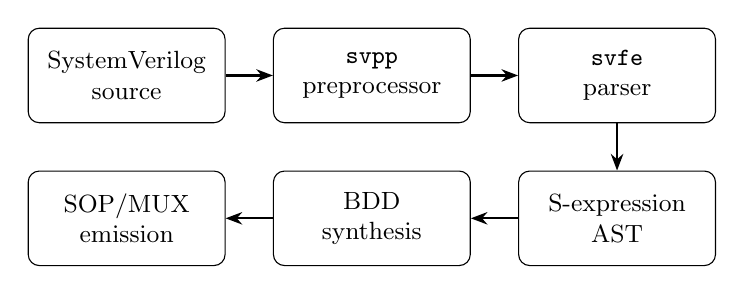
\begin{tikzpicture}[
  box/.style={draw, rounded corners, minimum height=1.2cm,
              minimum width=2.5cm, align=center, font=\small},
  arr/.style={-{Stealth[length=6pt]}, thick},
  node distance=0.6cm
]
\node[box] (sv) {SystemVerilog\\source};
\node[box, right=of sv] (pp) {\texttt{svpp}\\preprocessor};
\node[box, right=of pp] (fe) {\texttt{svfe}\\parser};
\node[box, below=of fe] (ast) {S-expression\\AST};
\node[box, left=of ast] (bdd) {BDD\\synthesis};
\node[box, left=of bdd] (sop) {SOP/MUX\\emission};

\draw[arr] (sv) -- (pp);
\draw[arr] (pp) -- (fe);
\draw[arr] (fe) -- (ast);
\draw[arr] (ast) -- (bdd);
\draw[arr] (bdd) -- (sop);
\end{tikzpicture}
\end{center}

The shell wrapper \texttt{run-svsop.sh} orchestrates the pipeline.
The \texttt{-{}-cut~N} flag sets the BDD cut threshold: intermediate
variables are introduced whenever a BDD exceeds $N$ nodes, keeping all
downstream BDDs bounded.

\section{The BDD Cut Mechanism}

When \texttt{*bv-cut-threshold*} is set to $N$, the function
\texttt{bdd-maybe-cut} replaces any BDD exceeding $N$ nodes with a
fresh variable, recording the definition in a global cut list:

\begin{lstlisting}[language=Lisp]
(define (bdd-maybe-cut bdd hint)
  (if (<= (bdd-size bdd) *bv-cut-threshold*)
      bdd
      (let* ((name (fresh-cut-name hint))
             (fresh (bdd-var name)))
        (record-cut! name bdd)
        fresh)))
\end{lstlisting}

Cut variables are emitted first as intermediate wire equations, then
the output equations reference them.  This keeps all equations bounded
in size.

Cuts are applied at three sites in the synthesis engine:
\begin{enumerate}
\item \textbf{Carry chains} --- after each bit of ripple-carry
  addition/subtraction/comparison
\item \textbf{Case decomposition} --- after each OR-accumulation step
  in the decoder+MUX architecture for large case statements
\item \textbf{If-else decomposition} --- after each priority-MUX
  accumulation step
\end{enumerate}

\section{The Blowup Problem}

\subsection{Symptom}

Running the SOP tool on the MOS~6502 CPU with \texttt{-{}-cut~30}
produced equations for most signals but hung indefinitely on the
processor status register bits \texttt{next\_P[7:0]}, particularly
bit~1 (the zero flag).

\subsection{Root Cause}

The 6502's combinational logic includes a \texttt{set\_nz} function
that sets the sign and zero flags from an 8-bit result:

\begin{lstlisting}[language=Verilog]
function [7:0] set_nz(input [7:0] val);
  set_nz    = P;
  set_nz[7] = val[7];          // sign flag
  set_nz[1] = (val == 8'd0);   // zero flag
endfunction
\end{lstlisting}

The zero flag is an 8-input AND of negated result bits:
\[
  Z = \overline{v_7} \cdot \overline{v_6} \cdot \overline{v_5} \cdot
      \overline{v_4} \cdot \overline{v_3} \cdot \overline{v_2} \cdot
      \overline{v_1} \cdot \overline{v_0}
\]

Each $v_i$ is a complex function of inputs (e.g., for ADC, $v_i$
depends on carry chains through all lower bits).  Even with carry cuts
at threshold~30, each $\overline{v_i}$ has ${\sim}30$ BDD nodes.
The \texttt{bv-eq} function computes this as a \texttt{fold-left} of
AND operations:

\begin{lstlisting}[language=Lisp]
;; Original: no cuts in accumulation
(list (fold-left bdd-and (bdd-true)
       (map (lambda (x y)
              (bdd-not (bdd-xor x y)))
            a1 b1)))
\end{lstlisting}

The AND-accumulation over 8 terms of ${\sim}30$ nodes each creates a
BDD that grows roughly as:

\begin{center}
\begin{tabular}{@{}lrr@{}}
\toprule
Step & Accumulator & BDD nodes \\
\midrule
$\overline{v_7}$ & $\overline{v_7}$ & $\sim$30 \\
$\overline{v_7} \cdot \overline{v_6}$ && $\sim$80 \\
$\overline{v_7} \cdot \overline{v_6} \cdot \overline{v_5}$ && $\sim$200 \\
$\vdots$ && $\vdots$ \\
$\prod_{i=0}^{7} \overline{v_i}$ && $\sim$2000+ \\
\bottomrule
\end{tabular}
\end{center}

This 2000-node BDD is then used as the body of each case arm.  When
the case decomposition OR-accumulates ${\sim}40$ arms (one per
opcode), the cut mechanism stores BDDs of 2000+ nodes---far too large
for efficient SOP conversion.

The SOP library's \texttt{invariantSimplify} has super-polynomial
worst-case complexity and hangs on these BDDs.  Shannon decomposition
(splitting on the top variable recursively) creates exponentially many
sub-equations.  Both approaches failed.

\subsection{Quantifying the Blowup}

The BDD size growth in the AND-accumulation is due to the cross-product
of variable orderings.  If each $\overline{v_i}$ depends on $k$
variables, and the variable sets partially overlap, the AND of $n$
terms can have up to $O(k^n)$ paths in the BDD.  For the 6502 zero
flag, $k \approx 30$ (8 data bits + 8 operand bits + carry cuts +
opcode bits) and $n = 8$, giving an effective BDD size in the
thousands.

\section{Solution: Syntax-Directed Decomposition}

\subsection{Cutting Inside Equality and Reduction}

The key insight is that the AND-accumulation inside \texttt{bv-eq}
must be cut, just like carry chains and case arms.  We add
\texttt{bdd-maybe-cut} at two levels:

\begin{enumerate}
\item \textbf{Input bits}: Cut each bit of the input bitvectors before
  forming XNOR terms, via a new helper \texttt{bv-maybe-cut-bits}:

\begin{lstlisting}[language=Lisp]
(define (bv-maybe-cut-bits bv hint)
  (if (not *bv-cut-threshold*) bv
      (map-indexed
        (lambda (i bit)
          (bdd-maybe-cut bit
            (string-append hint "_" (number->string i))))
        bv)))
\end{lstlisting}

\item \textbf{Accumulator}: Cut the running AND after each step:

\begin{lstlisting}[language=Lisp]
;; Fixed: cut accumulator at each step
(list (fold-left
        (lambda (acc xnor)
          (bdd-maybe-cut (bdd-and acc xnor) "eq"))
        (bdd-true)
        (map (lambda (x y)
               (bdd-not (bdd-xor x y)))
             a1 b1)))
\end{lstlisting}
\end{enumerate}

The same treatment is applied to the reduction operators
\texttt{bv-reduce-and}, \texttt{bv-reduce-or}, and
\texttt{bv-reduce-xor}.

With these cuts, the zero flag BDD stays bounded:

\begin{center}
\begin{tabular}{@{}lrr@{}}
\toprule
Step & BDD nodes & Cut? \\
\midrule
$\overline{v_7}$ & $\sim$30 & no \\
$\overline{v_7} \cdot \overline{v_6}$ & $\sim$50 & \textbf{yes} $\to$ 1 \\
$c_1 \cdot \overline{v_5}$ & $\sim$30 & no \\
$c_1 \cdot \overline{v_5} \cdot \overline{v_4}$ & $\sim$40 & \textbf{yes} $\to$ 1 \\
$\vdots$ & & \\
Final & $\sim$30 & \\
\bottomrule
\end{tabular}
\end{center}

\subsection{MUX Tree Emission}

For BDDs that exceed the SOP minimization threshold (50 nodes), we
emit a \emph{MUX tree}---a syntax-directed walk of the BDD structure.
Each decision node becomes one wire equation:

\[
  w_k = v \cdot w_{\text{hi}} + \bar{v} \cdot w_{\text{lo}}
\]

where $v$ is the decision variable and $w_{\text{hi}}$, $w_{\text{lo}}$
are the names assigned to the high and low children.

\begin{lstlisting}[language=Lisp]
(define (emit-mux-node prefix bdd)
  (cond
    ((bdd-true? bdd) "1'b1")
    ((bdd-false? bdd) "1'b0")
    ;; Leaf variable: hi=T, lo=F
    ((and (bdd-true? (bdd-high bdd))
          (bdd-false? (bdd-low bdd)))
     (bdd-name (bdd-node-var bdd)))
    ;; General: recurse, emit MUX equation
    (else
     (let* ((hi-name (emit-mux-node prefix (bdd-high bdd)))
            (lo-name (emit-mux-node prefix (bdd-low bdd)))
            (my-name (fresh-mux-name prefix)))
       (emit-equation my-name var hi-name lo-name)
       my-name))))
\end{lstlisting}

Properties of MUX tree emission:
\begin{itemize}
\item \textbf{Time}: $O(N)$ in BDD nodes (one equation per node)
\item \textbf{Space}: $O(N)$ intermediate wires
\item \textbf{Sharing}: Subgraph sharing via memoization---each unique
  BDD node is emitted exactly once
\item \textbf{Simplification}: Common cases are simplified:
  $v \cdot 1 + \bar{v} \cdot w \to v + w$;
  $v \cdot w + \bar{v} \cdot 0 \to v \cdot w$; etc.
\item \textbf{No SOP library}: No calls to \texttt{ConvertBool} or
  \texttt{invariantSimplify}---no risk of hanging
\end{itemize}

\subsection{Two-Tier Emission Strategy}

The final \texttt{emit-sop-eqn} function uses:

\begin{center}
\begin{tabular}{@{}lll@{}}
\toprule
BDD size & Strategy & Output format \\
\midrule
$\leq 50$ nodes & Minimized SOP & \texttt{a \& b | c \& d} \\
$> 50$ nodes & MUX tree & One wire per BDD node \\
\midrule
Constants & Direct & \texttt{1'b0} or \texttt{1'b1} \\
\bottomrule
\end{tabular}
\end{center}

\section{Results}

\subsection{MOS 6502 ALU}

The ALU is a pure combinational module with 15 operations.  With
\texttt{-{}-cut~30}:

\begin{center}
\begin{tabular}{@{}lr@{}}
\toprule
Metric & Value \\
\midrule
Cut variables & 70 \\
Output signals & 6 \\
Output bits & 14 \\
Max BDD size (at emission) & $\leq 50$ \\
Emission strategy & 100\% minimized SOP \\
Runtime & $\sim$30\,s \\
\bottomrule
\end{tabular}
\end{center}

All equations use minimized SOP---no MUX trees needed.

\subsection{MOS 6502 CPU}

The CPU has a 40-arm case statement decoding opcodes into register
updates.  With \texttt{-{}-cut~30}:

\begin{center}
\begin{tabular}{@{}lr@{}}
\toprule
Metric & Value \\
\midrule
Cut variables & 417 \\
Output signals & 18 \\
Output bits & 56 \\
Max BDD size (at emission) & 213 \\
Minimized SOP equations & 455 \\
MUX tree equations & 72 \\
Runtime & $\sim$30\,s \\
\bottomrule
\end{tabular}
\end{center}

All 56 output bits have equations, including the previously
intractable zero flag (\texttt{next\_P[1]}).

\subsection{Comparison of Approaches}

\begin{center}
\begin{tabular}{@{}llrrr@{}}
\toprule
Version & Strategy & Max BDD & Runtime & Completeness \\
\midrule
v1 & SOP only & 2900 & hung & 10/18 outputs \\
v2 & SOP + raw + skip & 2900 & $\sim$10\,min & 10/18 (8 skipped) \\
v3 & Shannon decomp & 2068 & hung & incomplete \\
v4 & MUX tree (no eq cuts) & 2327 & $\sim$5\,min & 18/18 \\
v5 & MUX tree + input cuts & 2068 & $\sim$3\,min & 18/18 \\
\textbf{v6} & \textbf{MUX tree + accum cuts} & \textbf{213} &
  \textbf{$\sim$30\,s} & \textbf{18/18} \\
\bottomrule
\end{tabular}
\end{center}

\subsection{Regression Tests}

All existing test suites continue to pass:

\begin{center}
\begin{tabular}{@{}lrr@{}}
\toprule
Test suite & Pass & Total \\
\midrule
BDD synthesis (8 modules) & 8 & 8 \\
Self-equivalence check & 8 & 8 \\
Round-trip verification & 7 & 8 \\
\bottomrule
\end{tabular}
\end{center}

The single round-trip failure (\texttt{test\_shift4}) is pre-existing
and unrelated to SOP changes.

\section{Example Output}

A representative output equation for the 6502 accumulator bit~7:

\begin{lstlisting}
next_A[7] = _cut_mux_next_A_7_244
  | A[7] & opcode[0] & opcode[1]
  | A[7] & opcode[1] & ~opcode[2] & opcode[4]
  | A[7] & ~opcode[0] & ~opcode[2] & ~opcode[3] & opcode[4]
  | A[7] & opcode[1] & ~opcode[2] & ~opcode[3] & opcode[6]
  | A[7] & ~opcode[0] & ~opcode[2] & ~opcode[3] & ~opcode[7]
  | ...
  // 16 products, 49 BDD nodes
\end{lstlisting}

The cut variable \texttt{\_cut\_mux\_next\_A\_7\_244} encodes the
opcodes that modify the accumulator (LDA, ADC, SBC, AND, ORA, EOR,
etc.)\ and is defined by its own set of equations earlier in the
output.

\section{Conclusion}

The key lesson is that BDD cut insertion must be applied not only at
the ``structural'' boundaries (carry chains, case arms) but also
inside \emph{expression-level} operations that accumulate over
multiple bits.  The equality operator \texttt{==} and reduction
operators (\texttt{\&}, \texttt{|}, \texttt{\^{}}) all perform
fold-left accumulations that can create BDDs exponentially larger than
their inputs.

The MUX tree emission strategy provides a reliable fallback for BDDs
too large for SOP minimization.  It is always $O(N)$ in BDD nodes,
produces correct equations, and avoids any dependency on the SOP
library's potentially super-polynomial minimization algorithms.

Together, these techniques make the SOP tool practical for real
designs: the full MOS~6502 CPU---a 40-arm case statement with 8-bit
arithmetic, carry chains, and flag computation---completes in 30
seconds with all outputs covered.

\end{document}
